%\documentclass[dvipdfmx]{beamer}      % platex の場合
\documentclass[handout]{beamer}        % lualatex の場合
\usepackage{mySld}
\usepackage{multicol}

\begin{document}
\title{基礎コンピュータ工学\\第5章 機械語プログラミング\\
       (パート7:繰り返し処理と比較命令)}
\date{}

\begin{frame}
  \titlepage
  \centerline{\url{https://github.com/tctsigemura/TecTextBook}}
  \vfill
  \centerline{本スライドの入手:
    \raisebox{-7mm}{\includegraphics[scale=0.3]{../Img/QRs5_7.png}}}
\end{frame}

%==============================================================================
%\begin{frame}
%  \frametitle
%  \tableofcontents
%\end{frame}

\section{繰り返し}
%==============================================================================
\begin{frame}
  \frametitle{繰り返し処理(1)}
  ループの最後で条件判断する例(Javaの do ... while に似ている)\\
  \vfill
  \centerline{\includegraphics[scale=0.7]{../Tikz/flow2.pdf}}
  \vfill
\end{frame}

%==============================================================================
\begin{frame}
  \frametitle{繰り返し処理(2)}
  ループの最初で条件判断する例(Javaの while に似ている)
  \vfill
  \centerline{\includegraphics[scale=0.7]{../Tikz/flow2C.pdf}}
  \vfill
\end{frame}

%==============================================================================
% \begin{frame}
%   \frametitle{繰り返しの例}
%   $1 + 2 + 3 + ... + 10$を計算する.(例題5-2)\\
%   \vfill
%   \begin{minipage}{0.47\columnwidth}
%     \centerline{\includegraphics[scale=0.55]{../Tikz/flow3.pdf}}
%   \end{minipage}
%   \begin{minipage}{0.52\columnwidth}
%     {\ttfamily
%       G0,G1,G2,SP が使用可能.\\
%       これらの役割を決める.\\
%       例えば次のように割り振る.
%       \begin{itemize}
%       \item G0:繰り返し回数のカウンタ
%       \item G1:足す数(1,2,3,...,10)
%       \item G2:合計(足される数)
%       \item G2 ← G2 + G1 はできない \\
%         次の2ステップに分解する.
%         \begin{itemize}
%           \item $[TMP] ← G1$
%           \item $G2 ←G2 + [TMP]$
%         \end{itemize}
%       \end{itemize}
%     }
%   \end{minipage}
%   \vfill
% \end{frame}

%==============================================================================
\begin{frame}
  \frametitle{繰り返しの例}
  $1 + 2 + 3 + ... + 10$を計算する.\\
  \vfill
  \begin{minipage}{0.26\columnwidth}
    \centerline{\includegraphics[scale=0.55]{../Tikz/flow3A.pdf}}
  \end{minipage}
  \begin{minipage}{0.36\columnwidth}
    {\ttfamily JZ使用(例題5-2)\\\scriptsize
      \begin{tabular}{|l|l|l|}
              & LD     & G0, N    \\
              & LD     & G1, ONE  \\
              & LD     & G2, ZERO \\
              &        &          \\
      LOOP    & ST     & G1, TMP  \\
              & ADD    & G2, TMP  \\
              & ADD    & G1, ONE  \\
              & SUB    & G0, ONE  \\
              & JZ     & STOP     \\
              & JMP    & LOOP     \\
              &        &          \\
      STOP    & ST     & G2, SUM  \\
              & HALT   &          \\
              &        &          \\
      N       & DC     & 10       \\
      ONE     & DC     & 1        \\
      ZERO    & DC     & 0        \\
      TMP     & DS     & 1        \\
      SUM     & DS     & 1        \\
    \end{tabular}}
  \end{minipage}
  \begin{minipage}{0.36\columnwidth}
    {\ttfamily JNZ使用(例題5-2改良版)\\\scriptsize
      \begin{tabular}{|l|l|l|}
              & LD     & G0, N    \\
              & LD     & G1, ONE  \\
              & LD     & G2, ZERO \\
              &        &          \\
      LOOP    & ST     & G1, TMP  \\
              & ADD    & G2, TMP  \\
              & ADD    & G1, ONE  \\
              & SUB    & G0, ONE  \\
              & JNZ    & LOOP     \\
              &        &          \\
              &        &          \\
              & ST     & G2, SUM  \\
              & HALT   &          \\
              &        &          \\
      N       & DC     & 10       \\
      ONE     & DC     & 1        \\
      ZERO    & DC     & 0        \\
      TMP     & DS     & 1        \\
      SUM     & DS     & 1        \\
    \end{tabular}}
  \end{minipage}
  \vfill
\end{frame}

%==============================================================================
\begin{frame}
  \frametitle{CMP(Compare)命令(比較命令)}
  レジスタの値とメモリの値を比較しフラグを変化させる.\\
  比較には引き算を使用する.
  \vfill
  \begin{description}
  \item[フラグ:] 計算結果により変化する.
    \vfill

  \item[ニーモニック:]\texttt{CMP GR,EA}~~~~~~~~~\texttt{(GR - [EA])}
    \vfill

  \item[命令フォーマット:] 2バイトの長さを持つ.\\
    \twoByte{$0101_2$}{\GR~\XR}{\A}
    \vfill

  \item[フローチャート:] 値を保存しない引き算の意味.\\
    \centerline{\includegraphics[scale=0.7]{../Tikz/cmp.pdf}}
  \end{description}
  \vfill
\end{frame}

%==============================================================================
\begin{frame}
  \frametitle{大小比較(演習問題の解答と同じ)}
  MとN大きい方を選択してLに格納する.\\
  \vfill
  \begin{minipage}{0.5\columnwidth}
    \centerline{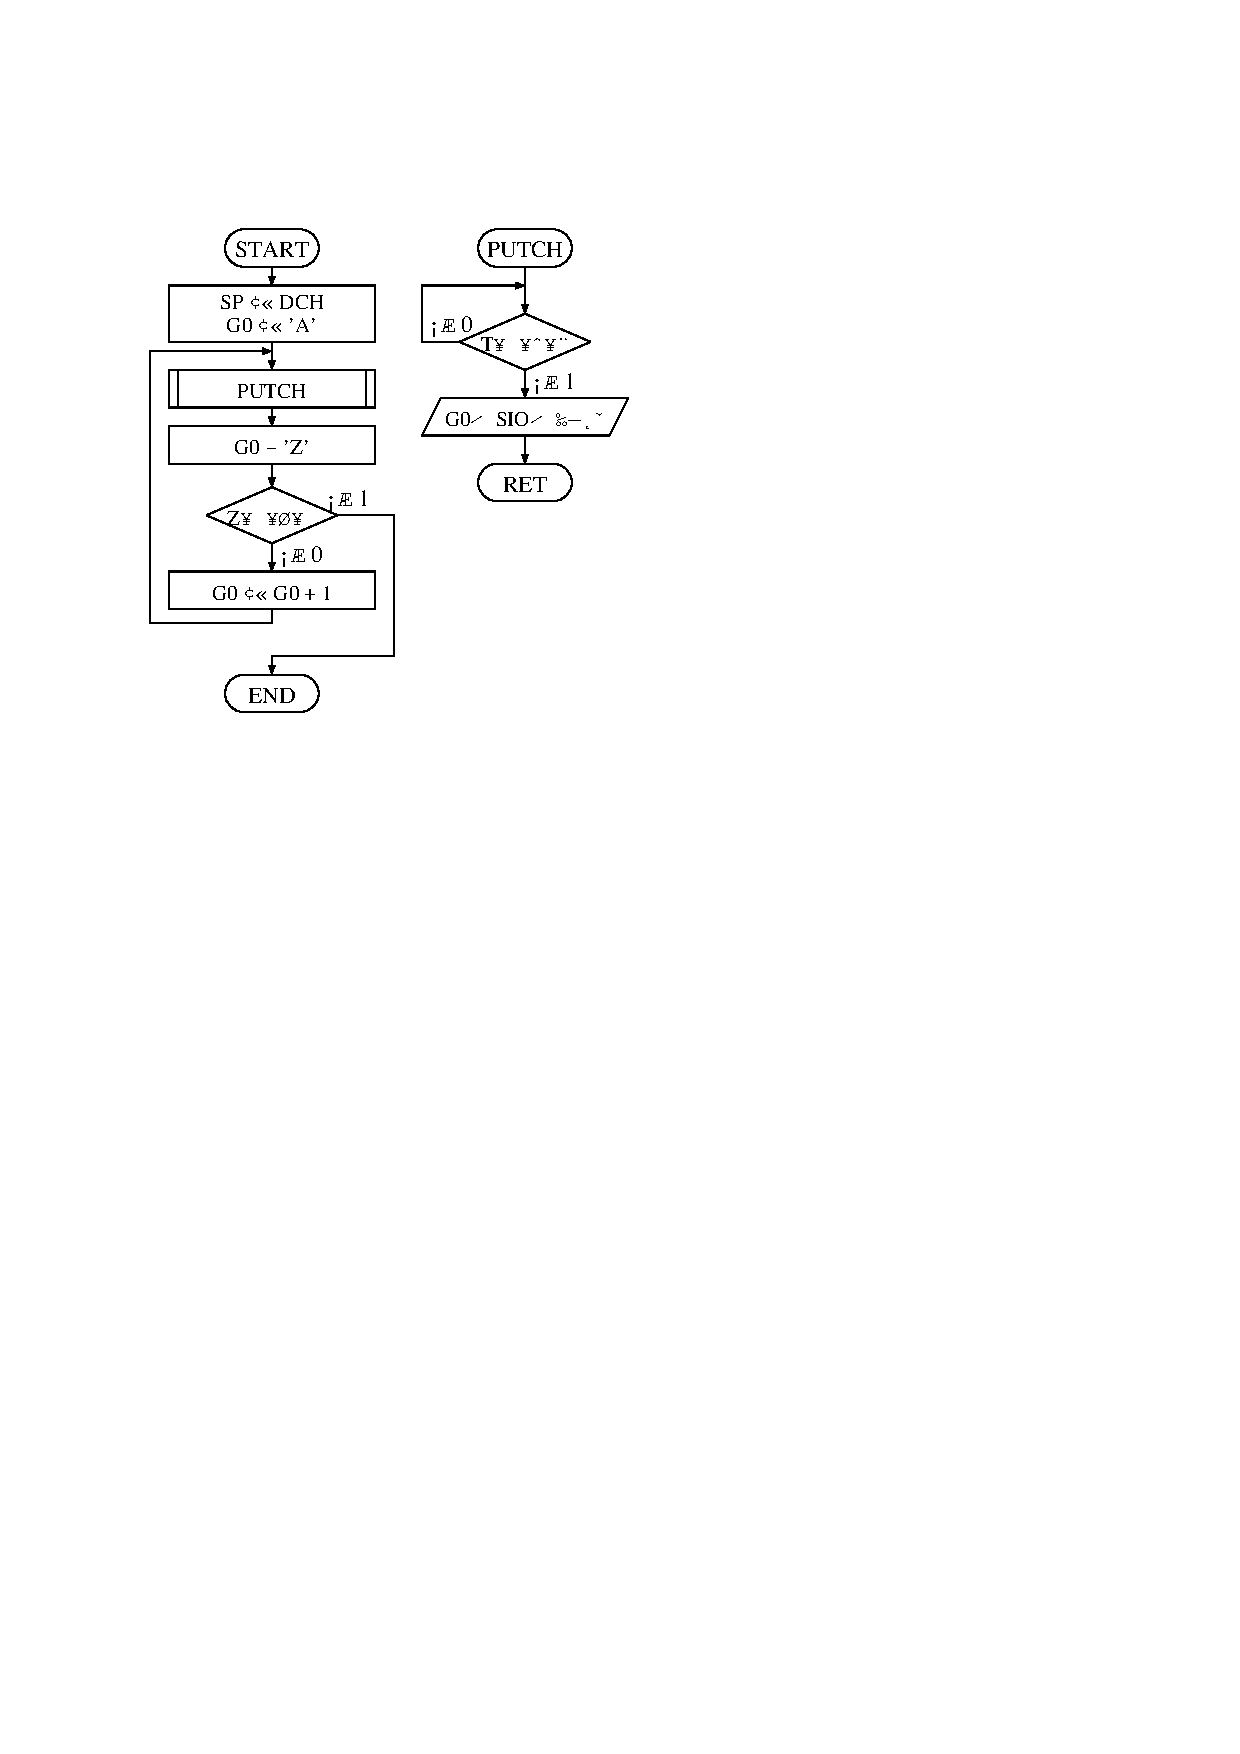
\includegraphics[scale=0.75]{../Tikz/flowI.pdf}}
  \end{minipage}
  \begin{minipage}{0.48\columnwidth}
    {\ttfamily\footnotesize
      \begin{tabular}{|l|l|l|}
              & LD     & G0, N    \\
              & SUB    & G0, M    \\
              & JM     & L1       \\
              &        &          \\
              & LD     & G0, N    \\
              & JMP    & L2       \\
              &        &          \\
      L1      & LD     & G0, M    \\
              &        &          \\
      L2      & ST     & G0, L    \\
              & HALT   &          \\
              &        &          \\
      N       & DS     & 1        \\
      M       & DS     & 1        \\
      L       & DS     & 1        \\
    \end{tabular}}
    \vfill
  \end{minipage}
\end{frame}

%==============================================================================
\begin{frame}
  \frametitle{大小比較(CMP,JNM 命令を使用して改良)}
  MとN大きい方を選択してLに格納する.\\
  \vfill
  \begin{minipage}{0.5\columnwidth}
    \centerline{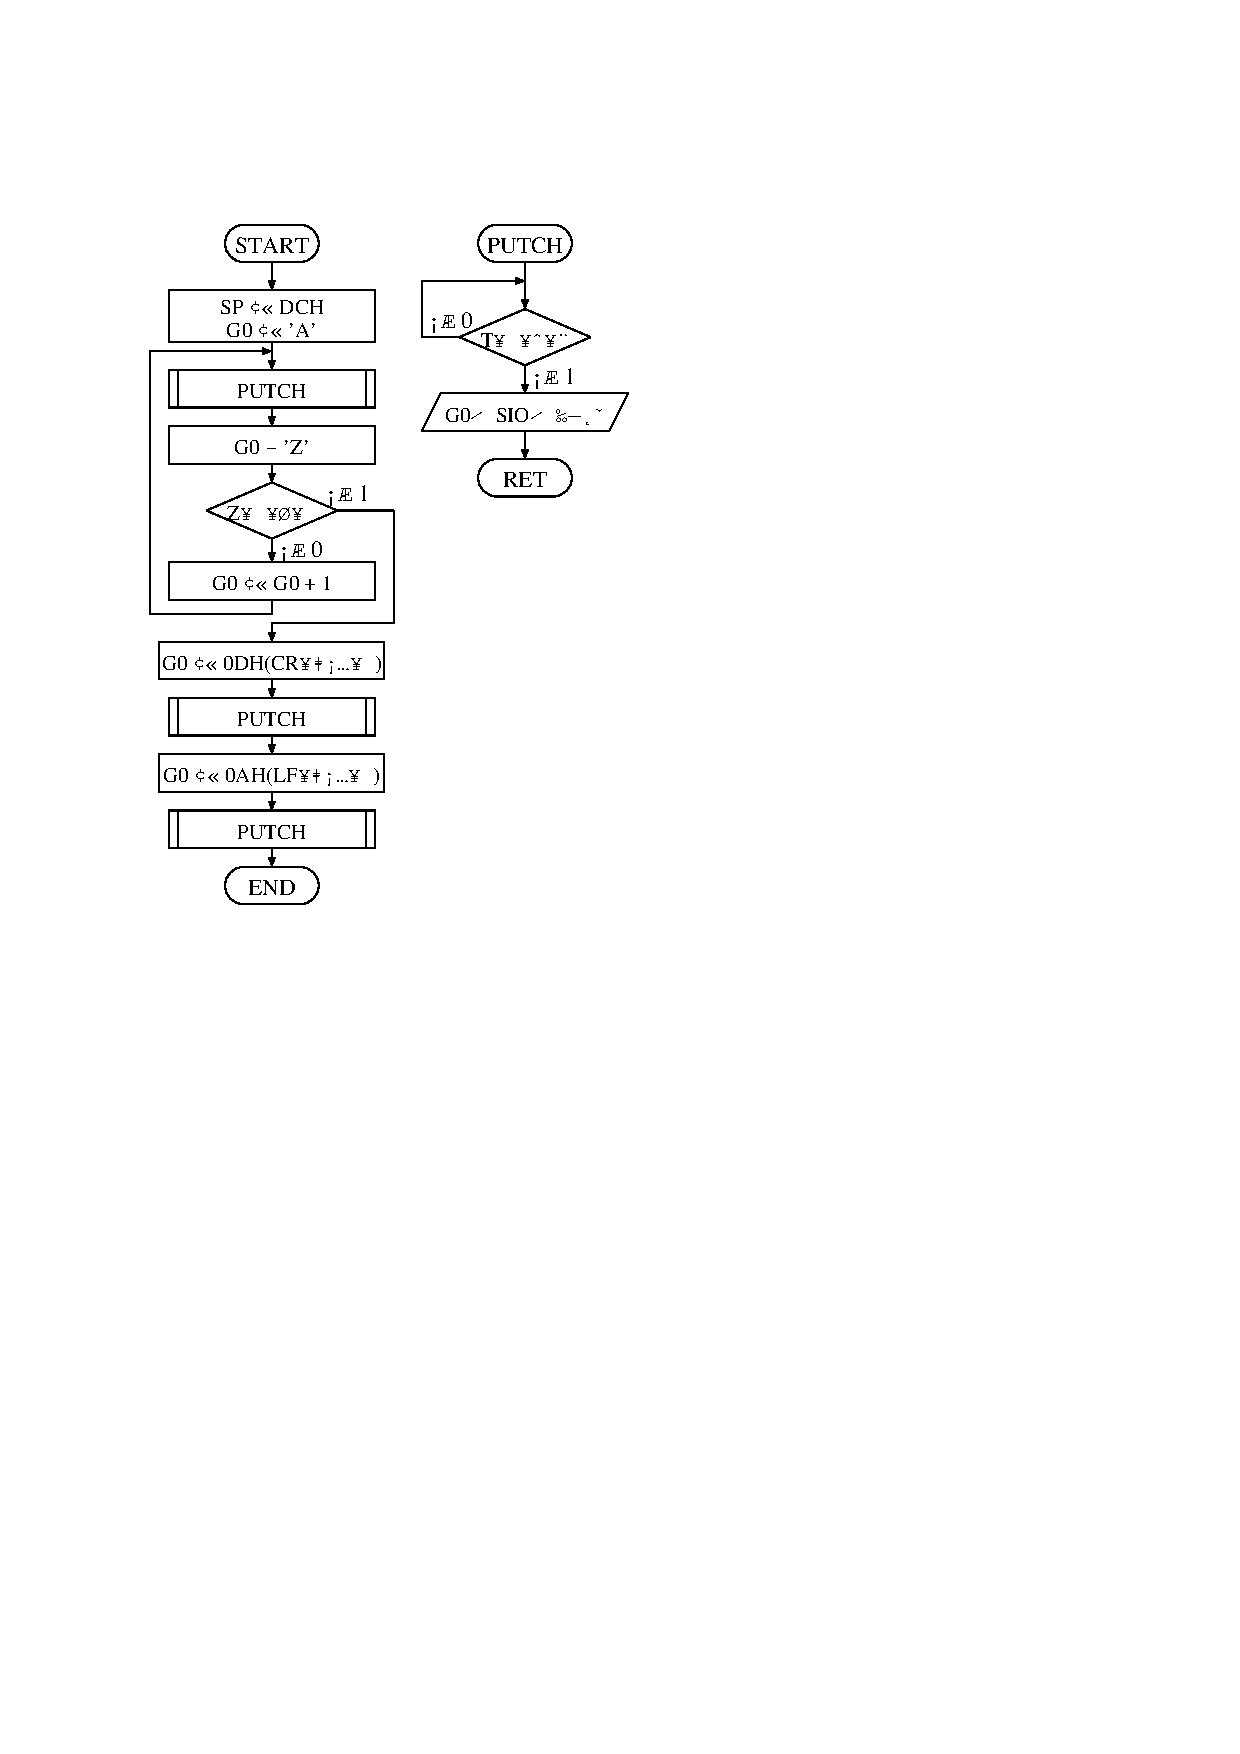
\includegraphics[scale=0.75]{../Tikz/flowJ.pdf}}
  \end{minipage}
  \begin{minipage}{0.48\columnwidth}
    {\ttfamily\footnotesize
      \begin{tabular}{|l|l|l|}
              & LD     & G0, N    \\
              & CMP    & G0, M    \\
              & JNM    & L1       \\
              &        &          \\
              & LD     & G0, M    \\
              &        &          \\
      L1      & ST     & G0, L    \\
              & HALT   &          \\
              &        &          \\
      N       & DS     & 1        \\
      M       & DS     & 1        \\
      L       & DS     & 1        \\
    \end{tabular}}
    \vfill
  \end{minipage}
\end{frame}

%==============================================================================
\begin{frame}
  \frametitle{まとめ}
  \emph{学んだこと}
  \begin{itemize}
  \item ループの作り方
  \begin{itemize}
    \item Javaのdo-whileに似たタイプ
    \item Javaのwhileに似たタイプ
    \end{itemize}
  \item 比較命令(CMP)
  \begin{itemize}
    \item 比較だけするときに役立つ.
    \item 引き算をしてみてフラグだけ変化する.
    \end{itemize}
  \end{itemize}
  \vfill

  \emph{演習(do-whileタイプのループ)}
  \begin{itemize}
  \item \emph{掛け算プログラム}:N番地のデータと,
    M番地のデータのかけ算を計算しL番地に格納するプログラム
  \item データはどれも符号なし整数とする.
  \item \color{red}繰り返し処理1のフローチャートを参考に作る.
  \end{itemize}
  \vfill
\end{frame}

%==============================================================================
\begin{frame}
  \frametitle{まとめ}
  \emph{演習(whileタイプのループ)}
  \begin{itemize}
  \item \emph{掛け算プログラム}:N番地のデータと,
    M番地のデータのかけ算を計算しL番地に格納するプログラム
  \item データはどれも符号なし整数とする.
  \item \color{red}繰り返し処理2のフローチャートを参考に作る.
  \end{itemize}
  \vfill

  \emph{演習(CMP命令)}
  \begin{itemize}
  \item \emph{割り算プログラム:}M番地のデータをN番地のデータで割り,
    商をK番地,余りをL番地に格納するプログラム
  \item データはどれも符号なし整数とする.
  \item 割り算は引き算の繰り返しでできる.
  \end{itemize}
  \vfill
\end{frame}

\end{document}
